%%
%% BIOTS - Hackathon 2018
%%
%% Roy Schubiger, 2018
%% 
%% Licence: Creative Commons Attribution-Share Alike 3.0 Unported
%% http://creativecommons.org/licenses/by-sa/3.0/
%% 

\documentclass[portrait,a4paper]{article}

\usepackage[utf8x]{inputenc}
\usepackage{amssymb, amsfonts, amsmath}
\usepackage{xcolor}
%\usepackage[e]{esvect}
\usepackage{floatrow} % allows to insert pictures into proofs and theorems

\usepackage{cancel}

\usepackage{graphicx}
%\usepackage{picins}
\usepackage{tabularx}
\usepackage{mwe} % for blindtext and example-image-a in example
\usepackage{wrapfig}
\usepackage{subfigure}
\usepackage{framed}
\colorlet{shadecolor}{orange!15}

\usepackage{geometry}
\geometry{a4paper, left=15mm, right=15mm, top=20mm, bottom=20mm} 

\usepackage{multirow}
\usepackage{multicol}
\columnsep24pt
\columnseprule0.1pt

\renewcommand{\baselinestretch}{1.4}

% hyperref
\usepackage[colorlinks=false,pdfborder = {0 0 0 0}]{hyperref}

\parindent0pt
\setcounter{secnumdepth}{4}

%% Redefine the \paragraph command:
\makeatletter
\renewcommand\paragraph{\@startsection{paragraph}{4}{0mm}%
	{-\baselineskip}%
	{0.5\baselineskip}%
	{\normalfont\bfseries}%
}%
\makeatother 

% algorithms
\usepackage{algorithmic}
\usepackage{algorithm}
\algsetup{linenodelimiter=}

% listings
\definecolor{darkgreen}{RGB}{0,127,14}
\usepackage{listings}

\usepackage{listings}
\usepackage{xcolor}
\lstset { %
    language=Java,
    backgroundcolor=\color{black!5}, % set backgroundcolor
    basicstyle=\ttfamily\mdseries, % basicstyle=\linespread{5},% basic font setting
    %escapeinside={!}{!},
    tabsize=4,
    morecomment=[l][\color{cyan}]{\#},
    % numbering
    numbers=left, stepnumber=1, numberstyle=\tiny, numbersep=20pt, numberblanklines=true,
    inputencoding=utf8x,
	xleftmargin=30pt,
	xrightmargin=10pt,
	aboveskip=0.5em,
    belowskip=0.5em,
    columns=fullflexible,
	breaklines=true,
	framerule=0mm,
	frame=single,
	showstringspaces=false,
	commentstyle=\color{black!65},	
	captionpos=b,
	float=float,
	mathescape= true
}
% theorem package
\usepackage{amsthm}
\usepackage{thmtools}
\newtheoremstyle{my-thm-style}% name
{6pt}% Space above
{5pt}% Space below
{}% Body font
{}% Indent amount
{\bfseries}% Theorem head font
{}% Punctuation after theorem head
{8pt}% Space after theorem head
{}% Theorem head spec (can be left empty, meaning `normal')
\definecolor{orange}{rgb}{1,0.5,0}
\declaretheoremstyle[
headfont=\normalfont\bfseries,
notefont=\mdseries, notebraces={(}{)},
bodyfont=\normalfont,
name={\ignorespaces},
headpunct=,
postheadspace=0pt,
spaceabove=1pt,
mdframed={
  skipabove=2pt,
  skipbelow=2pt,
  hidealllines=false,
  backgroundcolor={orange!40},
  innerleftmargin=8pt,
  innerrightmargin=8pt}
]{box}
\declaretheorem[style=box, numbered=no]{BOX}
\newcommand{\comment}[1]{\begin{BOX} #1 \end{BOX}}

\usepackage[english]{babel} 

\title{bEquality - Automated tracker for gender equality with blockchain \\[-10pt] Creation of an automated and reliable gender equality index}

\author{Qianchen Yu (TODO@student.ethz.ch), Lena Csomor (lcsomor@student.ethz.ch), \\[-4pt] 
Noah Berner (noberner@student.ethz.ch), Eric Léger (legere@student.ethz.ch),\\[-4pt] 
Fredin Thazhathukunnel (fredint@student.ethz.ch), Matthias Matti (mmatti@student.ethz.ch), \\[-4pt] 
Lino Telschow (tlino@student.ethz.ch), Roy Schubiger (roysc@student.ethz.ch) \\[10pt] 
ETH Z\"urich, 30.04.2018 \\[-16pt]}

\date{}

\begin{document}

\maketitle

\vspace{1pt}
\hrule
\vspace{1pt}

\begin{center}
	All contributors contributed equally to this report\\[8pt]
	The software code which is part of this report is open source and available at \url{https://github.com/ETHBiots2018/bEquality}\\[8pt]
	This project report was written as part of the spring 2018 course 'Blockchain And the Internet of Things (851-0591-01L)' run by M. Dapp, S. Klauser, and D. Helbing.\\[8pt]
	This report is licensed under a CreativeCommons licence CC BY-SA v4.0.
\end{center}

\vspace{1pt}
\hrule
\vspace{1pt}

\section*{Abstract}
	%introduction
	Today, most companies' market value is driven by intangible value, such as reputation or branch equity. 
	Thus, thousands of companies now provide detailed extra-financial information. 
	Regulations are mandating increased management disclosure and analysis on sustainability, and investors 
	are analyzing the comprehensive risks and opportunities of issuers in public and private markets. 
	One aspect of this extra-financial information is data on gender equality.\\
	And more and more investors take this data into consideration when investing as research suggests 
	that good gender equality practice can serve as an indicator for good corporate governance and decision 
	making and these companies might outperform in the future.
	%problem description
	To get a structured, concise and comparable overview of this data, investors often relay on established 
	gender-equality certifications. Unfortunately, this process is costly, time intensive and requires 
	multiple revisions to produce reliable data. 
	\footnote{This paragraph is taken from the challenge description handed to us by the UBS}\\

	%motivation	
	Our project aims to simplify and automate the process of obtaining such a gender-equality certifications 
	based on an existing Gender-Equality-Framework, and to make its results publicly accessible for everybody.\\
	%approach
	Our approach focuses on the data capture, data storage, data validation and a the display solution of the process.\\
	The data is obtained by the means of a website and an app whereas the storage solution relays on an 
	E-voting system, based on the latest blockchain and cryptographic technology. The solution provides 
	the code of the communication interfaces for the website and the app, as well as the necessary code 
	to handle the data for the E-Voting system via the blockchain.\\
	Furthermore, a Radar-Chart is used to present the results in a straightforward manner.\\

	%conclusion	
	In conclusion the platform ensures a trustful, transparent and cheap way to create a gender-equality-index, 
	which is useful for people to make investment decisions and for companies to further improve their status 
	with respect to gender equality.
	
	\subsection*{Introduction}
		The current situation of the economy is not fully inclusive for every member of the society, 
		women get discriminated, sexually harassed and do not have equal chance of high salaries and 
		or higher positions in companies.\\
		Our Project bEquality aims to punctually recognize inequality by providing a transparent, 
		reliable and efficient gender-equality index for companies. We think that applying and 
		evaluating a gender-equality index should not be expensive and exclusive to companies 
		that can afford it.\\
		We aim to improve todays state of society with respect to gender-equality in the economy.\\

		This document summarizes our approach to solve this problem. Our solution has come up on a hackathon 
		organized by the Blockchain and Internet of Things School (BIOTS) 2018.\\

		We will first present you our whole process systematically and then later dive further into the 
		implementation of the whole process.\\
		The reader should have basic programming understanding or basic logical thinking to understand 
		our approach and implementation, we try to explain it as easy as possible.

\section{Project}
	\subsection{Overview}
		\begin{figure}[H]
			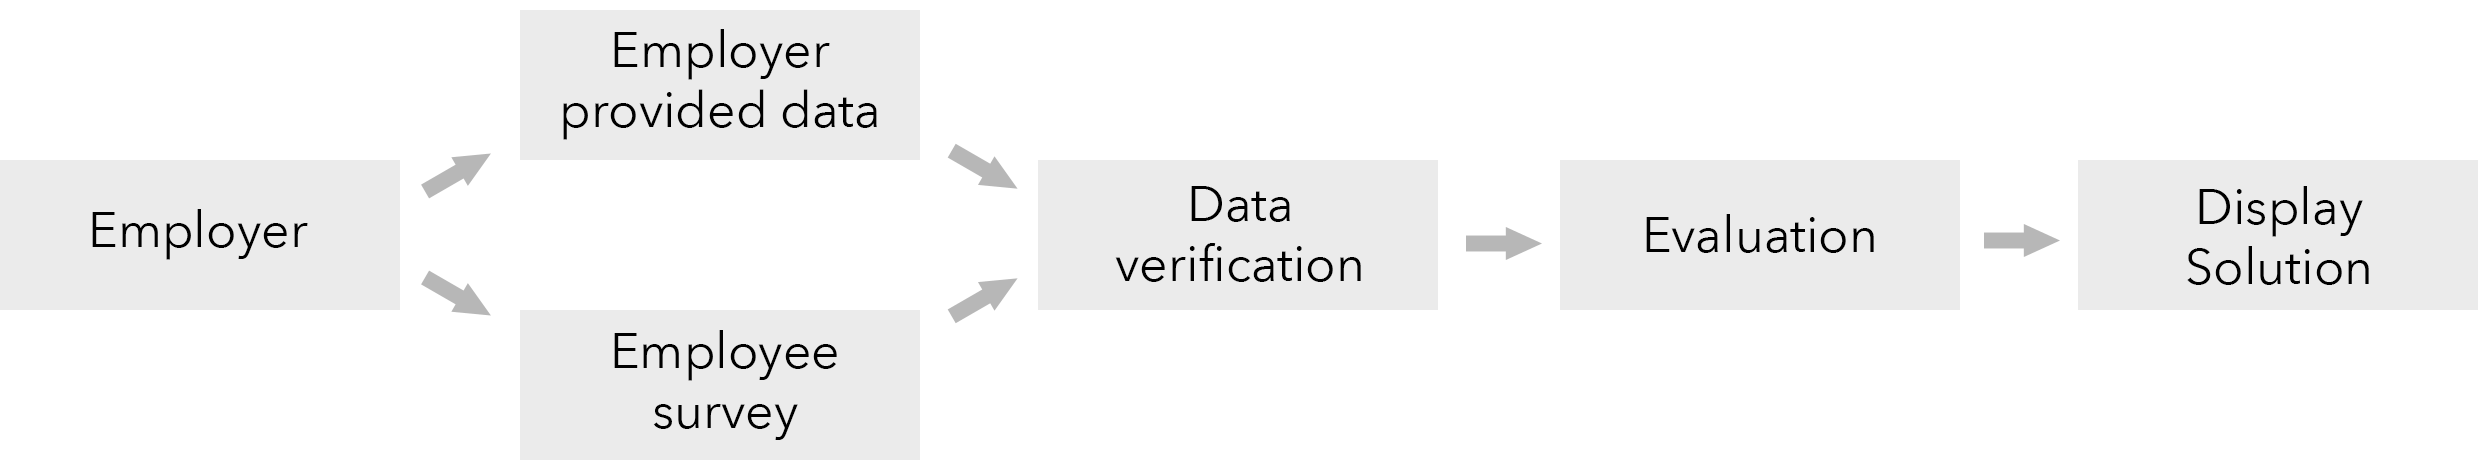
\includegraphics[width=0.9\textwidth]{Bilder/bEquality-Overview}
			\caption{Project flow graph}
			\label{Project_flow_graph}
		\end{figure}

		The figure \ref{Project_flow_graph} visualizes the high-level structure of our project.\\
		Existing gender-equality indices differ from our project at the points 
		\textit{data survey (employee survey)} and \textit{data} \textit{verification} 
		in the high-level structure and in the final evaulation.\\
		We will now explain the high-level structure of our project structure.

		\paragraph*{Employer Survey}
			There are a few necessary steps for an employer to get a certification.
			First, the employer has to to send the data asked for by the given rating 
			framework via a Website. Additionaly the company provides the E-mail-Addresses 
			of their employees. That’s the employer provided data.

		\paragraph*{Employee Survey}
			We will provide an employee survey to all employees of the company. 
			This survey is used to validate the plausability of the 
			provided data from the employer and to obtain further important private data 
			from employees that cannot be known by the employer.\\

			However, this is an easy task for the employee. To set up an account, the employee 
			gets an invitation link from our program and then gets linked to the app, 
			where he/she can set up his/her account. While setting up the account, 
			a public and a private key get generated in the background and linked to the employee account.\\
			After the account set-up the company sends all the public-keys generated by the employee 
			account set-up to our framework, this then initiates the survey set-up.\\
			When all background work is done, the employee gets a message that the survey 
			is ready. He/she has then just to log into the app, fill out the survey and then submit the data.\\

			Everything technical is handled automatically in the background, such that the 
			user just observes a handy interface, and all data is stored on either the blockchain or the IPFS.

		\paragraph*{Data Validation}
			When all data is gathered from all chosen employees, we split the data into different classes. 
			Either the data from the employees intersect the employer provided data, and is therefore 
			in the \textit{intersecting-data category}, or it is data that is just known or 
			provided by the employee (such as number of sexual harassments or similar things).\\

			All data from the \textit{intersecting-data category} gets compared by comparing the 
			provided view of the employer and the view of the employee.\\
			This comparison then provides a validity factor for the employer provided data.\\

			This process of data validation ensures that the data is not corrupted by either humans or bots.

		\paragraph*{Display Solution/Evaluation}
			We would adapt our evaluation to already existing gender-equality indices. 
			But to further improve these evaluations, we would like to evaluate also different indicators 
			for gender-equality and other measures that are important.\\
			The data evaluation then finally not just results in a single index number, but in a multidimensional 
			spider-diagram, that allows the investor or the company to look closer to existing problems or 
			advantages over the requirement.
			The figure \ref{Spider_diagram_evaluation__} provides a flexible evaluation system with detailed feedback.\\
			This detailed feedback is useful for company management and also useful for investment decisions 
			by investors that may want to invest in this company. It also implies a feedback system for the 
			company to rate, such that the company knows what to improve in it's employee environment to 
			further improve it's index.	
	
			
\section{Technical Implementation}
	
	\subsection{Data Capture and Storage}
		\paragraph*{Company Provided Data}
			As already mentioned earlier, the \textit{data capture} process is split into two parts.\\
			The first part consists of a survey that is sent to and filled out by the human resources 
			department of the company, i.e. the \textit{company provided data}.\\
			The questions on this survey will be based on already existing indices, 
			such as the ones from Bloomberg or Equileap.\\
			They fill out the survey directly on the website which stores the data on the blockchain via IPFS. 
			Because the data is stored directly on the blockchain, it is visible for everyone and 
			cannot be tempered with in any way at a later point in time.\\
			The company also sends us the email addresses of all their employees, which we will store 
			on a private and secure database. The email addresses can obviously not be stored on the 
			blockchain for privacy reasons. This is a tradeoff in transparency that was inevitable.

		\paragraph*{Employee Survey}
			The second part of \textit{data capture}, the \textit{employee survey}, is a special point of interest. 
			Because it is important to guarantee anonymity to the employee and at the same time ensure 
			validity and transparency of the data that is provided.\\

			The first step in the \textit{employee survey} takes part after we received all the email 
			addresses of the employees. We send them an email in which there is a link to our survey app.\\
			In the app, they enter a password for a new Ethereum blockchain account which gets 
			generated automatically. The private key of the account is stored only on the 
			employees device and is secured by the password they entered. The app sends the public address of the 
			blockchain to our server, where it is used to load a small amount of Ether onto it. 
			This is done, so that the employee can later make one transaction on the Ethereum blockchain.\\
			Once all the employees (or a big enough percentage) have followed our link and created an account, 
			our server will create a new survey contract on the blockchain.\\

			This happens via the following smart contract (contract \texttt{SurveyFactory}), 
			where an array of public addresses and a hash to the location of the addresses in IPFS is 
			required to create a new smart contract of the kind \texttt{Survey}.\\[-4pt]
			\begin{lstlisting}
// https://github.com/ETHBiots2018/bEquality/blob/master/Survey.sol
/*	SurveyFactory serves as a hub 
	(deployed on the blockchain upon the launching of bEquality)
	Company can create their own survey by providing a list of permitted user address. */

contract SurveyFactory {
  mapping(uint => address) public SurveyContracts;
  ...
  function createNewSurvey(uint companyID, address[] addressessOfEmployees, string _hashToaddressessOfEmployees) public returns(address newContract)
  {
    require(SurveyContracts[companyID] == 0x0);
    Survey c = new Survey(addressessOfEmployees, _hashToaddressessOfEmployees);
    SurveyContracts[companyID] = c;
    return c;
  }
  ...
 }
			\end{lstlisting}
			\texttt{SurveyFactory} can be thought of as a container in which all the surveys of the 
			different companies are stored and can be accessed via the unique id of the company.

			After the \texttt{Survey} contract is created, the employees are notified that they now can 
			fill out the survey. They log into their account on the app and answer the questions provided by us. 
			This is done via a user-friendly interface \footnote{A possible user-friendly interface can be found
			in the appendix}.\\
			The survey for the employees presents them with gender specific questions and also with questions 
			applicable for both men and women. These questions guarantee further insight into the microclimate 
			of the employees that cannot be obtained by just consulting the company management.\\
			When they submit the data, it gets stored on IPFS and the hash is again stored on the blockchain.\\
			This is done via the smart contract \texttt{Survey} seen below. It takes a hash to the location of the 
			survey results on IPFS and stores it on the blockchain.\\[-4pt]
			\begin{lstlisting}
// https://github.com/ETHBiots2018/bEquality/blob/master/Survey.sol
/*
   Survey is the child contract created by the SurveyFactory where only the permitted user can modify.
*/

contract Survey {
    mapping (address => string) public hashes;
    mapping (address => bool) public isAllowedToSumbitSurvey;
    string hashToaddressessOfEmployees;

    function Survey(address[] addressessOfEmployees, string _hashToaddressessOfEmployees) public {
        hashToaddressessOfEmployees = _hashToaddressessOfEmployees;
        for (uint256 index = 0; index < addressessOfEmployees.length; index++) {
            isAllowedToSumbitSurvey[addressessOfEmployees[index]] = true;
        }
    }

    function submitResults(string myHash) public {
        require(bytes(hashes[msg.sender]).length == 0);
        require(isAllowedToSumbitSurvey[msg.sender]);
        hashes[msg.sender] = myHash;
    }
}
			\end{lstlisting}
			The contract ensures that only the employees addresses which were submitted on contract creation 
			can submit results. It also ensures that an employee can only submit results once and that 
			he/she can not alter any other results.\\
			Because the employee knows his/her own public blockchain address (it is displayed on the app), 
			he/she can easily verify that the data on the blockchain did not get altered by anybody.\\
			The employee is also the only person who knows that this public key is associated to him/her. 
			Thus the sensitive data stored publicly on the blockchain still insures the privacy of the employee 
			and the employer cannot prosecute the employee for telling his opinion on the company.\\

			In our implementation most of the data that gets collected is only stored indirectly on the 
			blockchain via IPFS hashes. This was necessary to reduce the costs of the individual transactions 
			and for overall scalability.\\
			Ethereum transaction costs depend, among other things, on the size of the data stored on the blockchain. 
			If we only store hashes instead of survey data, the size of the transaction remains small, 
			no matter the number of questions in the survey.\\

			There are still challenges ahead of us for improving our implementation. For example the possibility of 
			storing the public Ethereum addresses on the blockchain instead of a private database while they are 
			still being collected for further transparency and automation of the process.

		\paragraph*{App Implementation}
			To make the survey as easy as possible for the employees, we decided to use an app. 
			We built a demo app for Android smartphones with the Android Studio IDE. \footnote{A visual preview
			of this APP can be found in the appendix}\\
			The app is only a concept and should serve as a visual guide of how the actual working app would look like. 
			Our demo app consists of a sample survey and dummy buttons and cannot actually submit the survey to the blockchain.\\
			Because of the limited time, we were not able to build a working app. Besides the time factor, we did not 
			know how to link the app with the Blockchain/IPFS and if there even is a Java interface to accomplish this task.\\
			Nevertheless, our app serves as a great visual reference.\\

			The fully implemented app could then work as follows:
			\begin{enumerate}
				\item	The employee sees a login screen and is asked to fill in his password for the Ethereum blockchain account.
				
				\item 	Once logged in, the app shows the user the questions to answer. 
						The interface is straightforward and self-explanatory.
						
				\item	After the user submits the survey, the app sends the survey results to the Blockchain/IPFS 
						and reports that the submission was successfull. 
						It also shows the employee his/her blockchain address for verification purposes.
			\end{enumerate}

			The big advantage of an app is the self explanatory user interface.\\

			Some of the disadvantages of using an app to collect data are:
			\begin{itemize}
				\item 	Even for one survey, the app needs to be installed on the phones of the employees.
				
				\item	Survey questions are hard-coded into the current app.
			\end{itemize}
			The second problem can be solved by downloading the questions from a server after the user is logged in. 
			With this approach the app serves as a framework for all kinds of surveys.\\

			It is unforeseeable if the app is the right choice to use for the gender equality survey and 
			a good way to find out if it is, would be to test multiple different ways of collecting data 
			and then analysing their effectiveness.
				
	\subsection{Data Verification}
		As already mentioned in the overview part, we can distinct our data into three different categories:
		\begin{itemize}
			\item	solely employer data
			\item	Intersecting data
			\item	solely employee data
		\end{itemize}
		We cannot prove the validity of the solely employer data, neither the validity of the solely employee data, because 
		we do not have access to a reference data set to compare it.\\
		Whereas we can look at the plausibility of the intersecting data provided by the employee, by comparing
		it to the reference data set provided by the employee.\\
		
		The objective of our data verification process is to provide a number that represents the plausibility
		of our evaluation.\\
		One approach to obtain such a number is the following process described below.\\
		
		When looking at the intersecting data category and then look at two specific subsets.
		One subset, say $A$, is provided by the employer. The other subset, say $B$, is provided by the employees.\\
		In our survey we have different questions or other measures that can represent the answers. One now could categorize
		these answers as a number between 1 and 10 (this could also be done more fine-grained or more coarse-grained).
		These numbers should be set in advance, such that they represent a goodness measure of the answers with respect
		to the order of the given numbers.\\
		With this insight, one now can represent the data in $A$ and the data in $B$ respectively, by a vector with
		$n$ dimensions, where $n$ is the number of questions or important measures (this obviously depends on the survey).\\
		Let's say the corresponding vector to the data set $A$ is called $a$, and $b$ to the set $B$ respectively.\\
		As a validity measure of the data in $A$, one now could take the following number:
		\begin{equation*}
			{\left\Vert a - b \right\Vert}^{2}
		\end{equation*}
		It represents the norm of the difference of the two vectors squared. This performance measure would punish 
		differences in the dimensions more than similarity in the respective dimension.\\
		
		As an improvement one could also represent this result as a number between 0 and 1, by eventually norming the
		vectors $a$ and $b$ in advance, and then representing the result as a percentage value for validity. But this
		process could be implemented in a more advanced state of the project.\\
		
		Please note, that this is just an approach of data verification measure, and that there are other measures that
		follow the objective, that are maybe better than this approach.
		
	\subsection{Display Solution/Evaluation}
		Currently, gender equality barometers, as the Bloomberg Gender Equality Index or the Equileap Ranking, 
		display the result of each company as a single number, score or grade. With this information, 
		a consumer (e.g. an investor) can see which company performs cares about gender equality or which 
		company is "'more"' gender equal than another one. But this one-dimensional approach does not offer 
		a lot more insight.\\
		A consumer of such a ranking is probably not only interested that a company makes effort 
		in gender equality, but also \textbf{how} they do.
		Moreover, to see how a single number (e.g. the rating result) -which includes a lot of different factors- is composed, 
		it requires quite a bit of investigation.
		To address these points, our display solution focuses on a multidimensional approach by means of spider diagrams.
		\begin{figure}[H]
			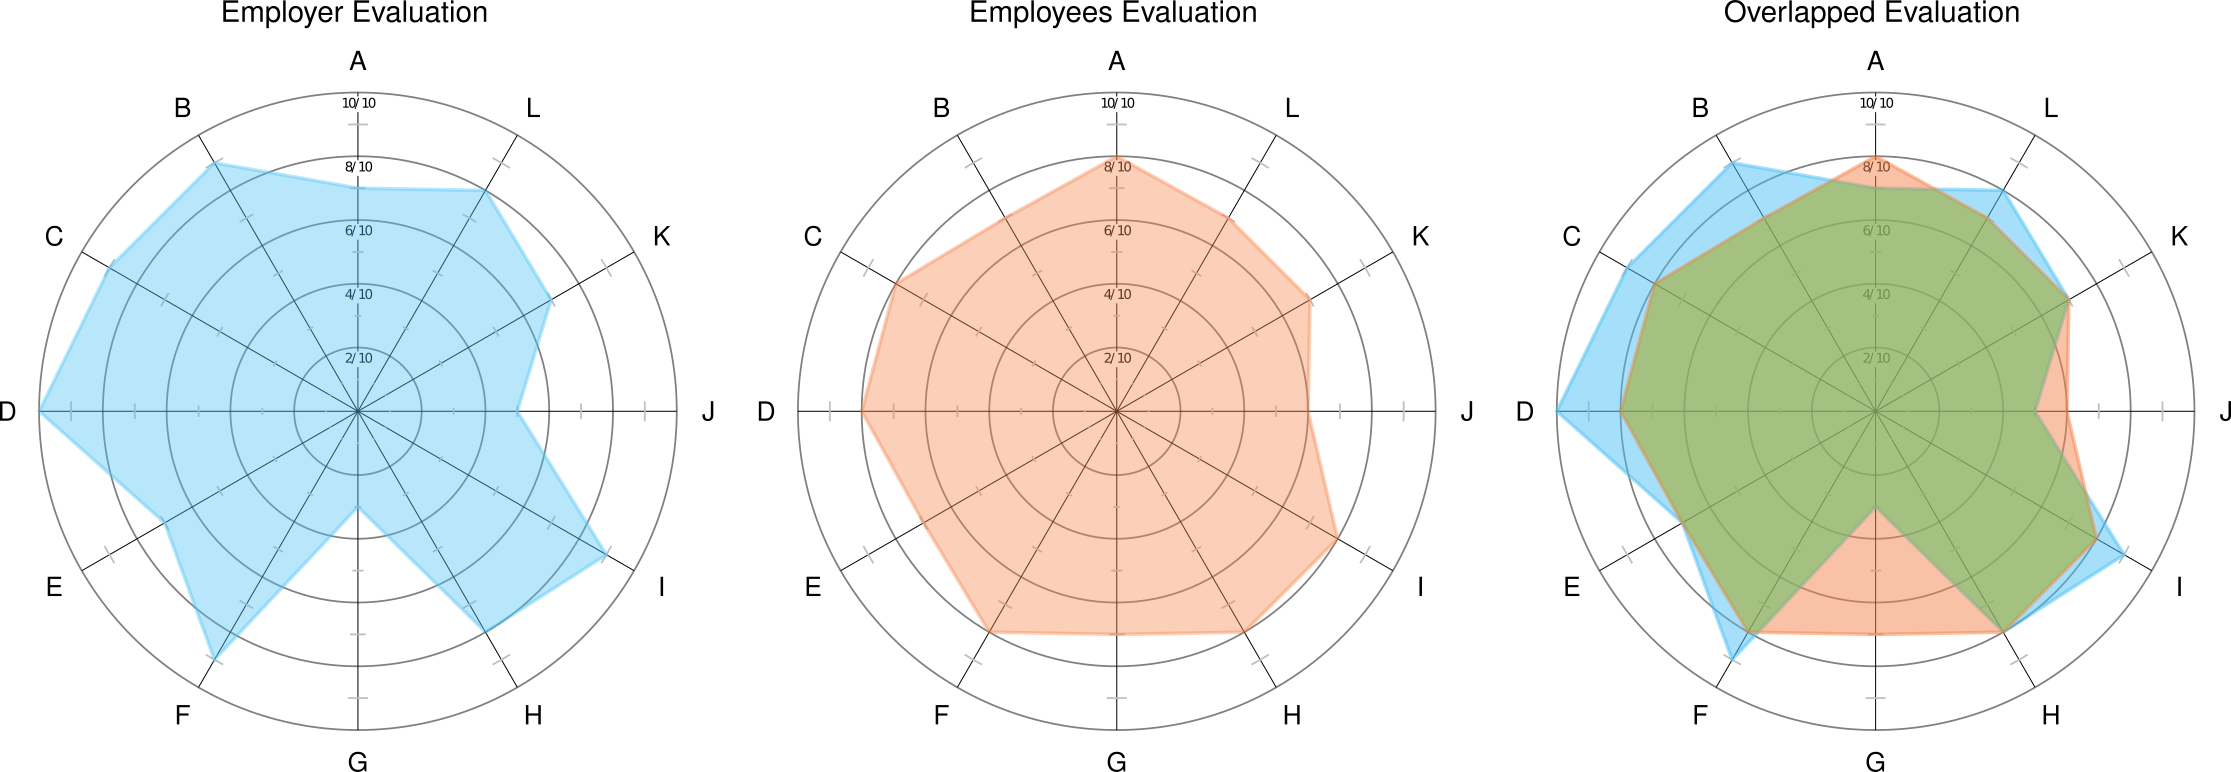
\includegraphics[width=0.95\textwidth]{Bilder/spider-eval}
			\caption{Spider-diagram evaluation example}
			\label{Spider_diagram_evaluation__}
		\end{figure}

		With the spider diagram it is possible to show multiple factors at the same time. One each branch of the 
		diagram a different factor can be displayed (in the figure, the labels 'A - L' represent each one factor.\\
		An important in the survey evaluation is to identify the relevant factors which should be included 
		into the spider diagram. These factors could rely on the existing frameworks ( e.g. from Bloomberg or Equileap) 
		or one could come up with new factors based on the surveys. An obvious factor is for sure the 
		difference of salaries between men and women for equal performances.\\
 
		Due to the settings of the surveys, there will be data from the employer survey which can not be caputered 
		by the employee survey and vice versa. For example, the employer can deliver factual data, whereas the 
		employee can express his personal impressions and experiences of the daily work life. 
		This data can be boundled in the \textit{non-intersecting-data category}. Nevertheless, concerns, 
		which are addressed in both surveys can be compared. This data can be boundled in the \textit{intersecting-data category}.\\
		As shown schematically in the figure above, these two categories can be in an straigtforward 
		manner with spider diagrams. On the one hand, the \textit{non-intersecting-data category}, there could 
		be a spider diagram for the employer survey as well as the employee survey. 
		On the other hand, a spider diagram with the \textit{intersecting-data category} 
		could present the factors, where data from both sides is displayed.\\

		The overlapping in the spider diagram of the \textit{intersecting-data category} can serve as an 
		indicator of data-validity. When a company provides wrong data, then this would result in a smaller overlapp. 
		One has to take into account, that people could be forced by the company to give certain answers 
		to gain a competitve advantage. \footnote{An approach to solve this problem can be found in the data verification section}\\

		Since spider diagrams are widely known, and the display solution is easy to read. 
		Due to the fact that the diagram displays more than a number as the other ratings, 
		it is a nice tool to gain additional, comprehensible insight into the efforts a company does 
		in the field of gender equality.\\

		Because the data from the evaluations is open accessible on IPFS, the diagrams can easily be generated and 
		fetched from these places and be displayed via a website or an app.

	\subsection{Challenges to solve and further points worth to consider}
		There are still some challenges to solve for this project.\\
		
		% implement E-Voting
		One major challenge is to provide a secure way of implementing a system equivalent to E-voting, 
		i.e. to find a system where a user applies to a survey or evaluation and the data provided by 
		him cannot be traced back to this user, even when the user can verify that the data provided 
		by him is used and not some modified version of his data.\\
		A way of solving this problem for this use-case (of a gender-equality index) it may be a 
		solution to implement the system in such a way, that cheating for companies are too expensive 
		to be profitable and the company therefore acts cooperatively and provides true data.\\
		Once we are certain that the company does not cheat we have to look at the behaviour 
		of those who can have a great impact on the evaluation: the employees.\\
		
		% Survey participation
		We have to assume that the participation rate of the employee survey is rather low, 
		surely not more than 50 percent. This is because people who are moderately happy often 
		do not feel like they have to praise their employer, but they also do not complain. 
		Therefore, most of the people who will respond are either unhappy or very happy, 
		the votes of the moderate people get lost. To get a useful a participation rate, 
		this means we have to send emails to every employee.\\
		We have to be certain that with our questions, we get the information we really want. 
		They have to be detailed and unambiguous. Furthermore, we have to adapt the questions for 
		different hierarchy levels. A manager may have other concerns than a worker.
		To not lose the participator's interest, we have to make sure that the questions are short, 
		easy to understand and that there are not too many of them.\\
		
		% Easy and anonym questions
		Also, it is our concern that there is no (easy) way to identify the voter by his answer. 
		A rather simple way to avoid part of it is the strategy of randomised response. 
		This means that if two people are at the exact same point in the survey, let's say they both 
		have two choices to tick, one may be asked a trivial question, like which sort of ice cream he likes. 
		The other one will be asked a serious question which is important for out data collection. 
		This way, even if someone knows at which point which choice has been made, (for example he sees 
		the employee ticking on his smartphone, but cannot read the question from a distance) 
		he does not know what it meant.\\
		We know that anonymising data opens the door for abusers who try to manipulate the survey. 
		The more anonymous the participation is, the easier it is to abuse it. Sadly we have not yet found a 
		way to fix this completely - we can only agree on a certain balance between control and anonymity.\\
		
		% what questions
		An other problem we had was to determine which questions we should take for the survey in the application. 
		The application on the mobile phone should actually be a small survey for the employee to fill in with around 
		5 minutes. But there are a lot of questions we have to ask in order to get useful data which can be 
		compared with the data we got from the head of the companies. With enough participants, a random selection of questions 		for each employee could be a solution.\\
		
		% what indicators
		A similar issue is to find fitting indicators that are best to display in the Radar-Chart-Diagram, that provides
		enough useful information worth to consider, and at the same time does not abstract away some useful information.
		This indicators should also allow to compare different companies that are on our index, even if they do not have
		an equal number of employees or act in different industries.\\
		
		% costs with blockchain
		Another challenge is to handle and predict the costs to create a contract and store some data on the blockchain.
		These costs should, when it is possible, be avoided by some more efficient and cheaper approaches with
		the same advantages as our approach has.\\
		
		% better log-in process
		One problem we encounterd and couldn't solve, was the login process for the employees. 
		Our current implementation depends on, that each employee has to create his own account before taking the survey.
		The obvious disadvantage of this solution is, that each employee needs to remember his personal password. 
		A better approach would be an automated login process, such that the blockchain account is set up in the
		background. With this approach the password may be created randomly, without the users knowing about.\\

		% finish implementation
		Also because of the lack of time we couldn't finish our implementation completely. 
		The Mobile Applications needs to collect the data and put the collected data onto the block-chain.


\section{Conclusion}
	\paragraph*{Strengths and weaknesses}
		Our solution provides a reliable, transparent and automatic way of creating a gender-equality index. 
		Compared to other already existing indexes we offer an index where the reliability and correctness 
		can be verified by each and every person. This is done by implementing our strategy on the block-chain.
		
		Our approach allows everybody to classify companies according to the latest law regulatory for gender-equality in companies.
		
		Our solution is multidimensional, where multidimensional stands for two different things. 
		First of all our index contains different categories where the result is weighted and then demonstrated 
		as a graph \ref{Spider_diagram_evaluation__}.
		The other multidimensionality of our project is that we collect data from two different sources. 
		We collect it from the managers and we collect the data from a casual worker as well.
		
		A great advantage over existing gender-equality indices is that our solution is public and can be implemented
		with low costs. Existing indices nowadays require a lot of work e.g. to collect the data, to evaluate the data, 
		to present the data in a meaningful way and so on. In our solution we are trying to do as much as possible in an automatic approach.
		
		A downside of our approach, is that we need to send an invitation link to every employee to ensure enough participation and
		at the same time create a blockchain account for every participant before he/she can take the survey.

	\paragraph*{Open Challenges}
		There are several ways to expand our project. Examples would be to achieve a full working automatic way of 
		indexing gender-equality. This is our main idea but we haven't completed the implementation.\\
		The application we use to do the survey has just an interface. This means that we should collect the data on 
		the application and try to put the collected data onto the block-chain for further calculation processes.\\
		We still did not come up with a perfect system to verify a persons identity, neither did we find a good solution to
		this online. There are many different open challenges to improve our E-voting system, such that we can guarantee data 
		validity as well as anonymity for the participant.
		Every Survey that is submitted, corresponds to a block-chain transaction. This can get very expensive, since surveys can 
		contain alot of data. Our idea was to store the Survey results on an IPFS storage and only transmit the hash over the 
		block-chain. Therefore we need a greater understanding of IPFS and how to implement such a system into our application.
		
	\paragraph*{Disruptional Potential}
		Our approach is revolutionary in the sense that our process is completely transparent and every step in our process
		can be observed by the employee as well as by the investors.\\
		As well as we guarantee data availability for the employees as well as for investors, such that they can
		examine their own results from the given and anonymized data on the blockchain.\\
		
		And finally, our system allows a reliable and transparent way to improve gender-equality and in the long term
		decrease gender discrimination or discrimination that follows other incentives.
		
\section{Sources and Literature}
 	% Dateiname - Author - Jahr - Link/Buch\\
	Sources used in order to develop the app we used:
	\begin{itemize}
		\item https://developer.android.com
		\item https://stackoverflow.com
	\end{itemize}
	

\clearpage


\section{Appendix}
	
	\subsection{Survey-App prototype}
		Below is an App-prototype. From left to right is the Log-in screen, two survey screenshots and the screen, when the
		employee has succressfully submitted his/her answers to the blockchain / private database.
		\begin{figure}[!htb]
			\minipage{0.24\textwidth}
  				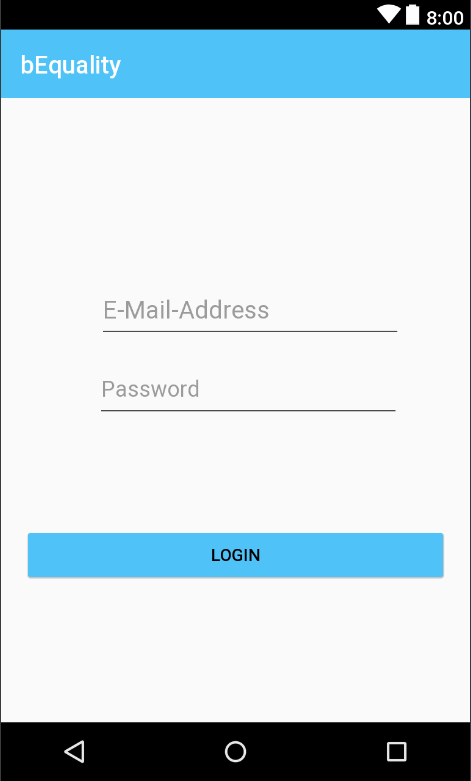
\includegraphics[width=\linewidth]{Bilder/App_1_Log-in}
  				
			\endminipage\hfill
			\minipage{0.24\textwidth}%
  				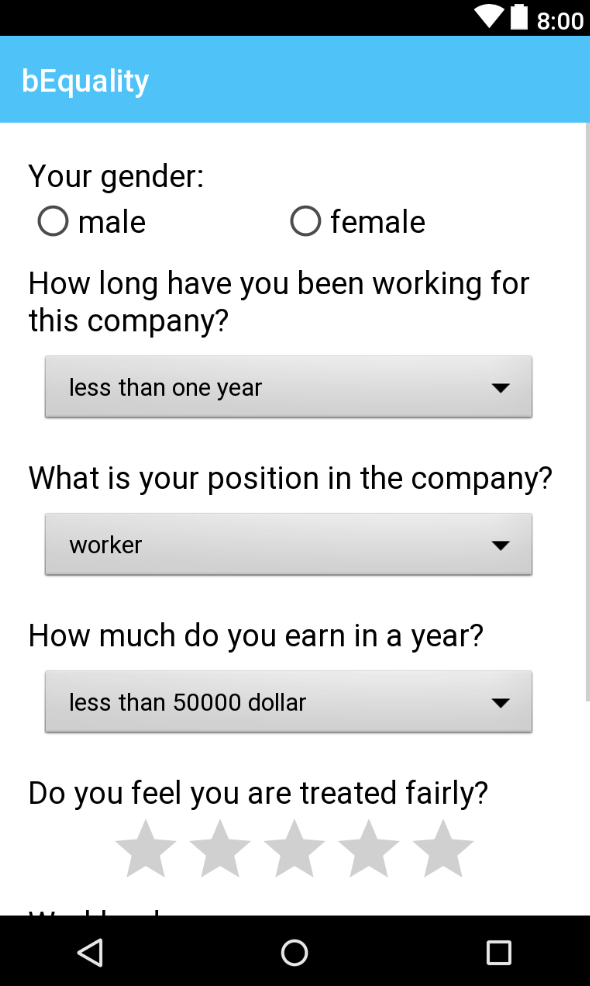
\includegraphics[width=\linewidth]{Bilder/App_2_Survey_1}
  			
			\endminipage\hfill
			\minipage{0.24\textwidth}%
  				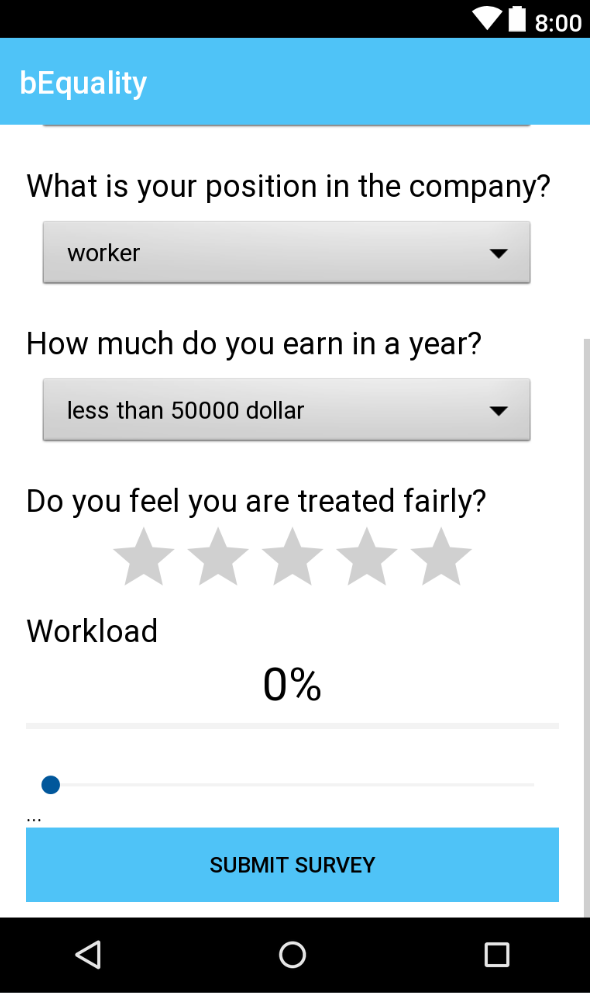
\includegraphics[width=\linewidth]{Bilder/App_3_Survey_2}
  				
			\endminipage\hfill
			\minipage{0.24\textwidth}%
  				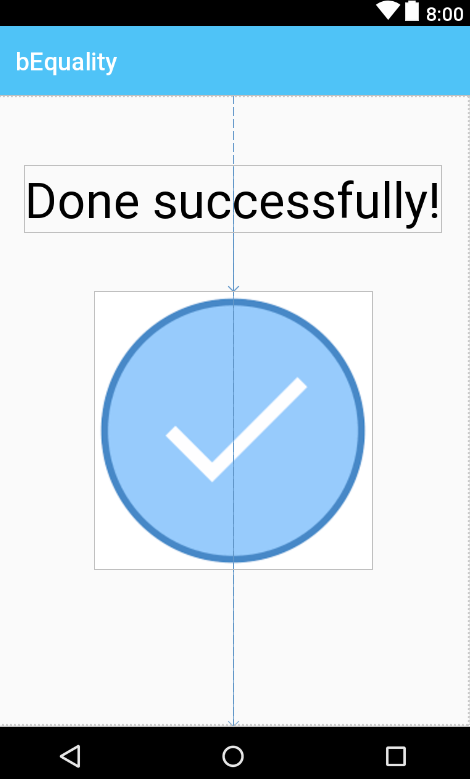
\includegraphics[width=\linewidth]{Bilder/App_4_lastpage}
  				
			\endminipage
		\end{figure}
		
	\subsection{Web interface}
		As an alternative to the Survey-App, we also implemented a website prototype, that can communicate with the blockchain
		and store the survey data on the blockchain.\\
		Here is a short overview of this website-prototype, for further insight, one can download the source code of this website.
		\begin{center}
			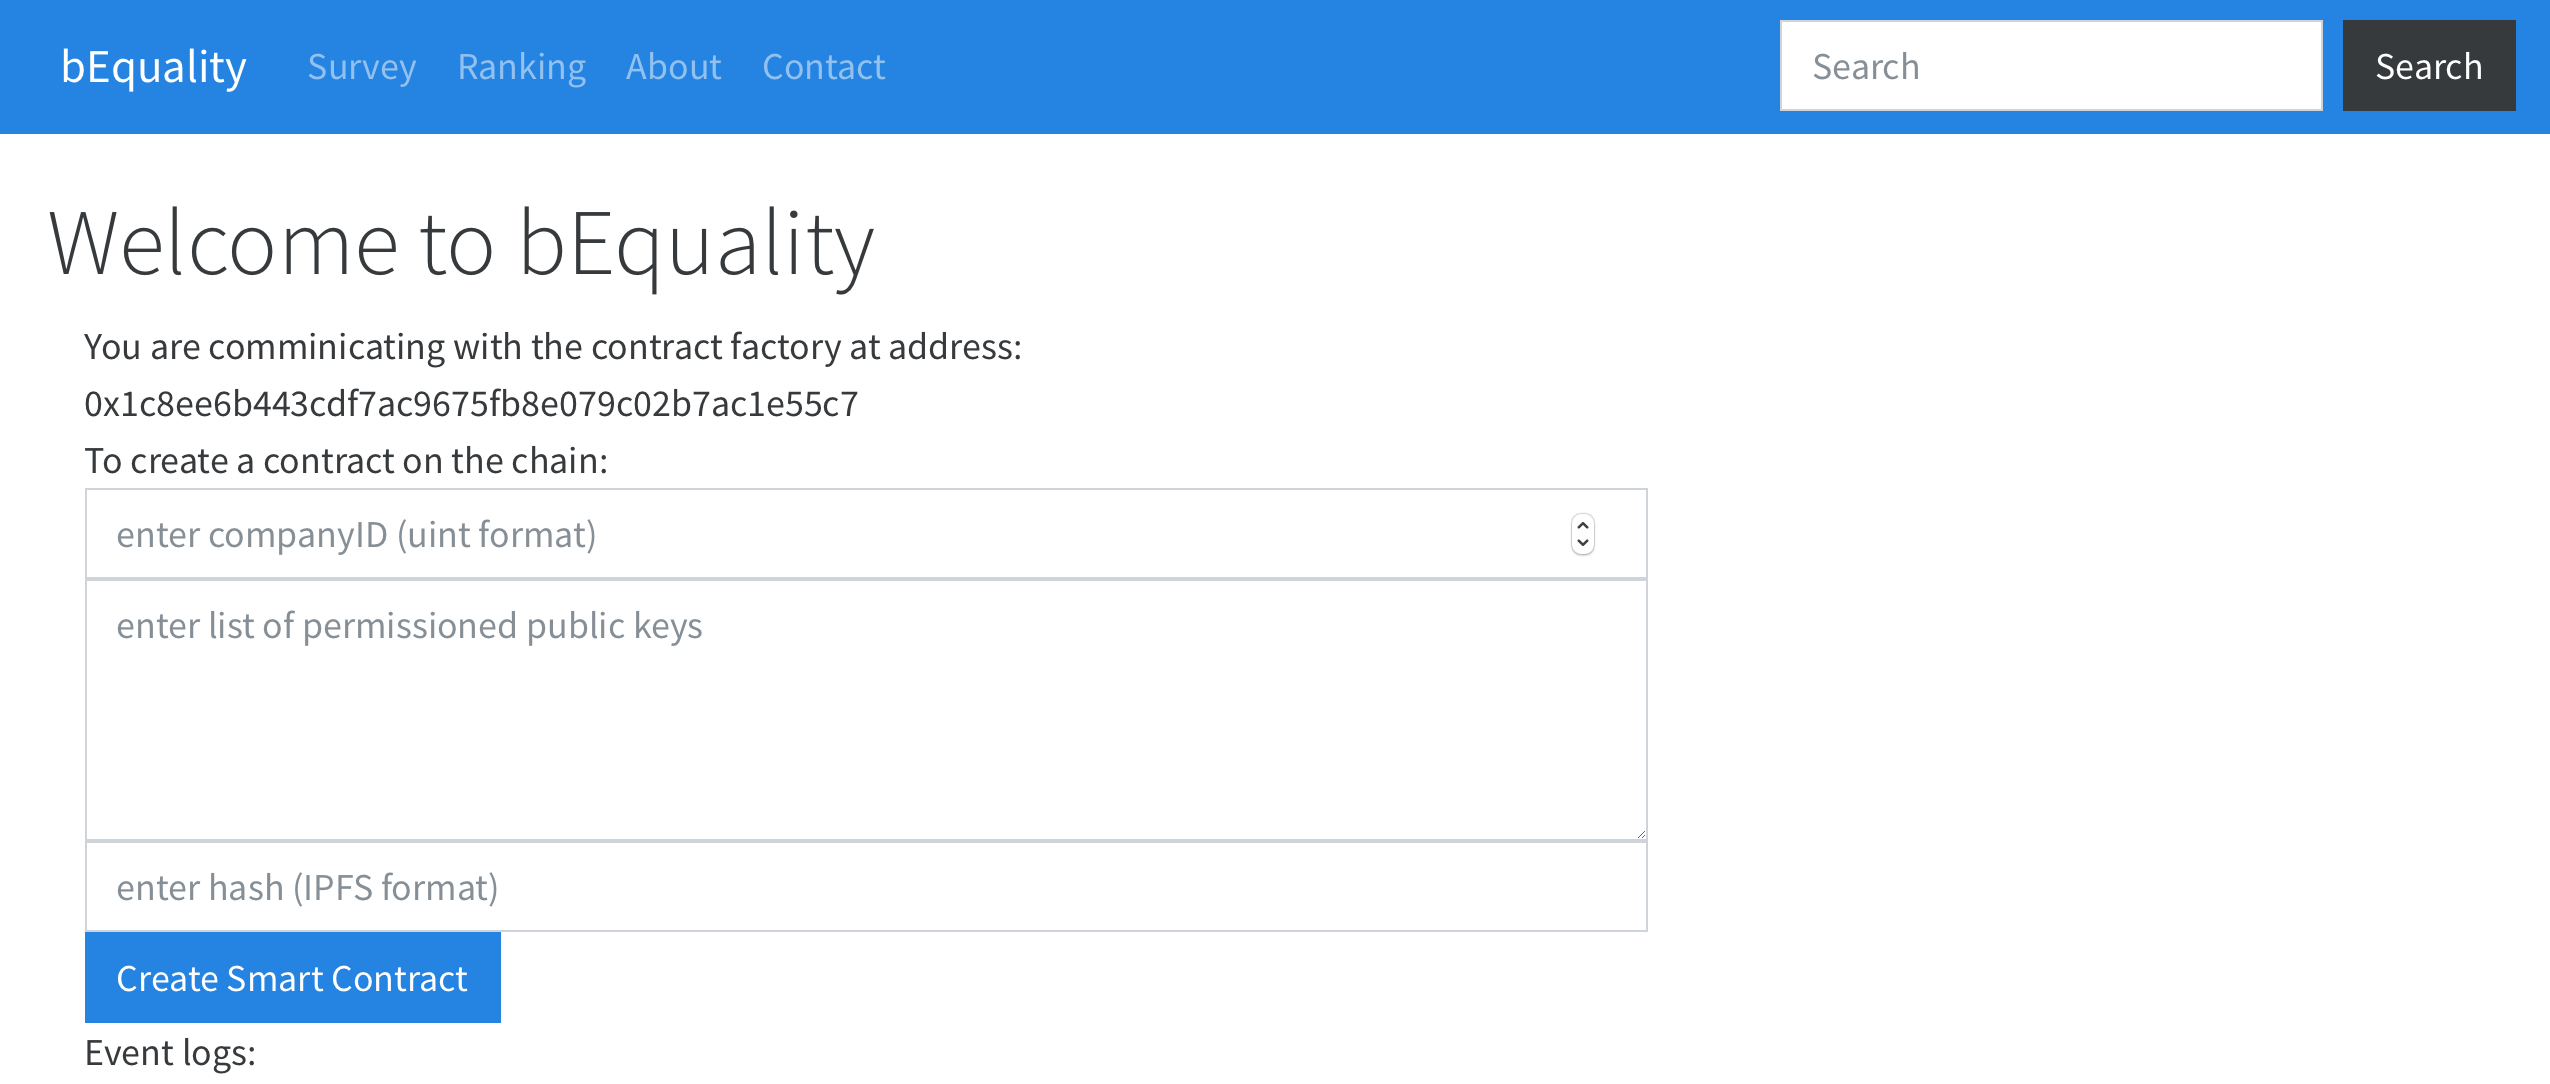
\includegraphics[width=0.7\textwidth]{Bilder/Website_1}
		\end{center}
		\begin{center}
			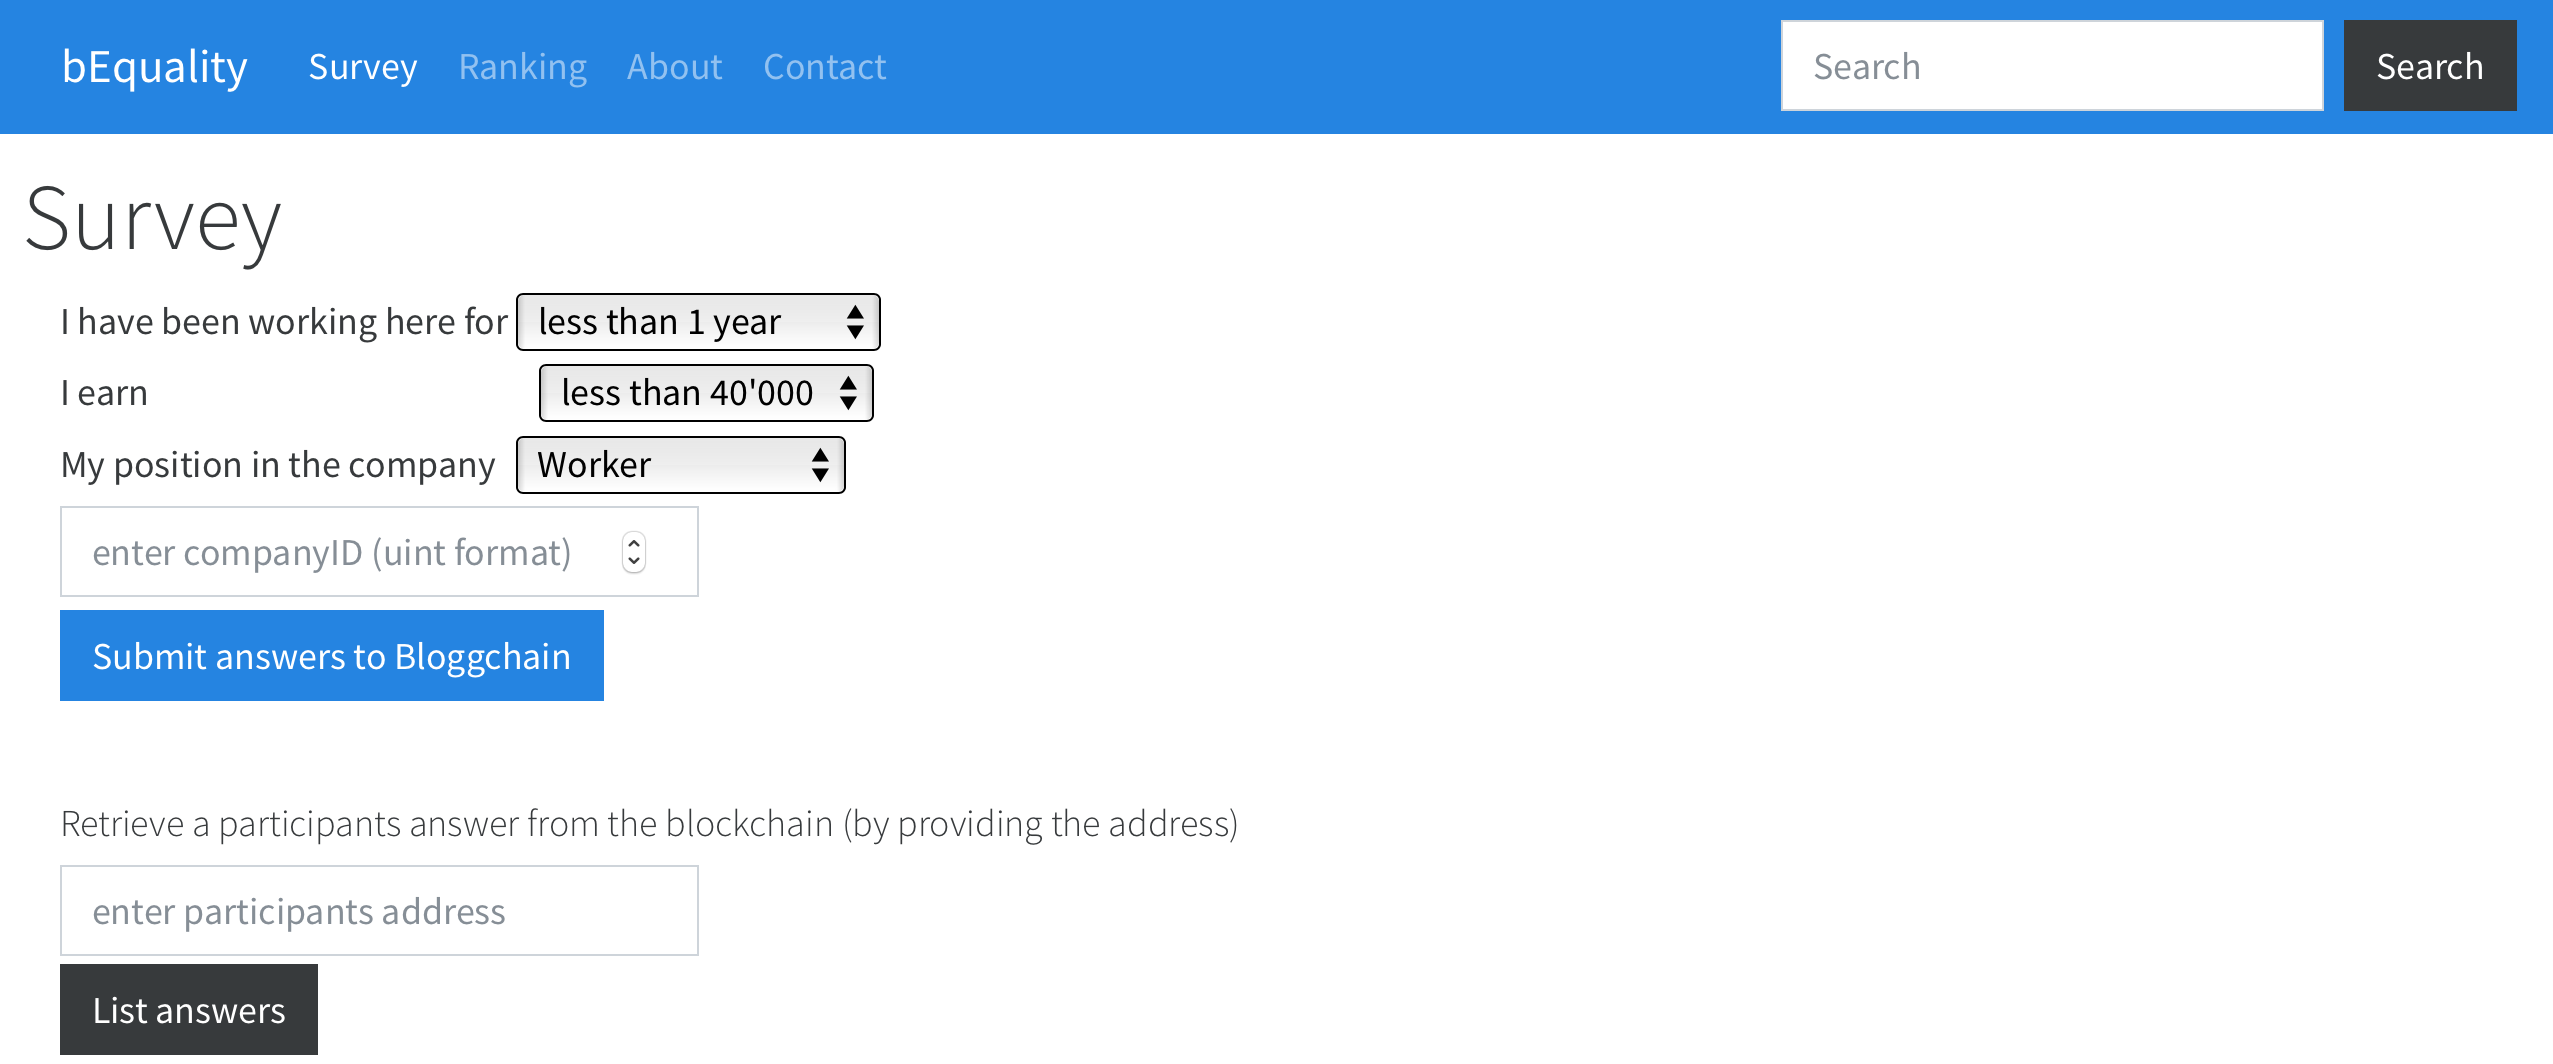
\includegraphics[width=0.7\textwidth]{Bilder/Website_2}
		\end{center}
		\begin{center}
			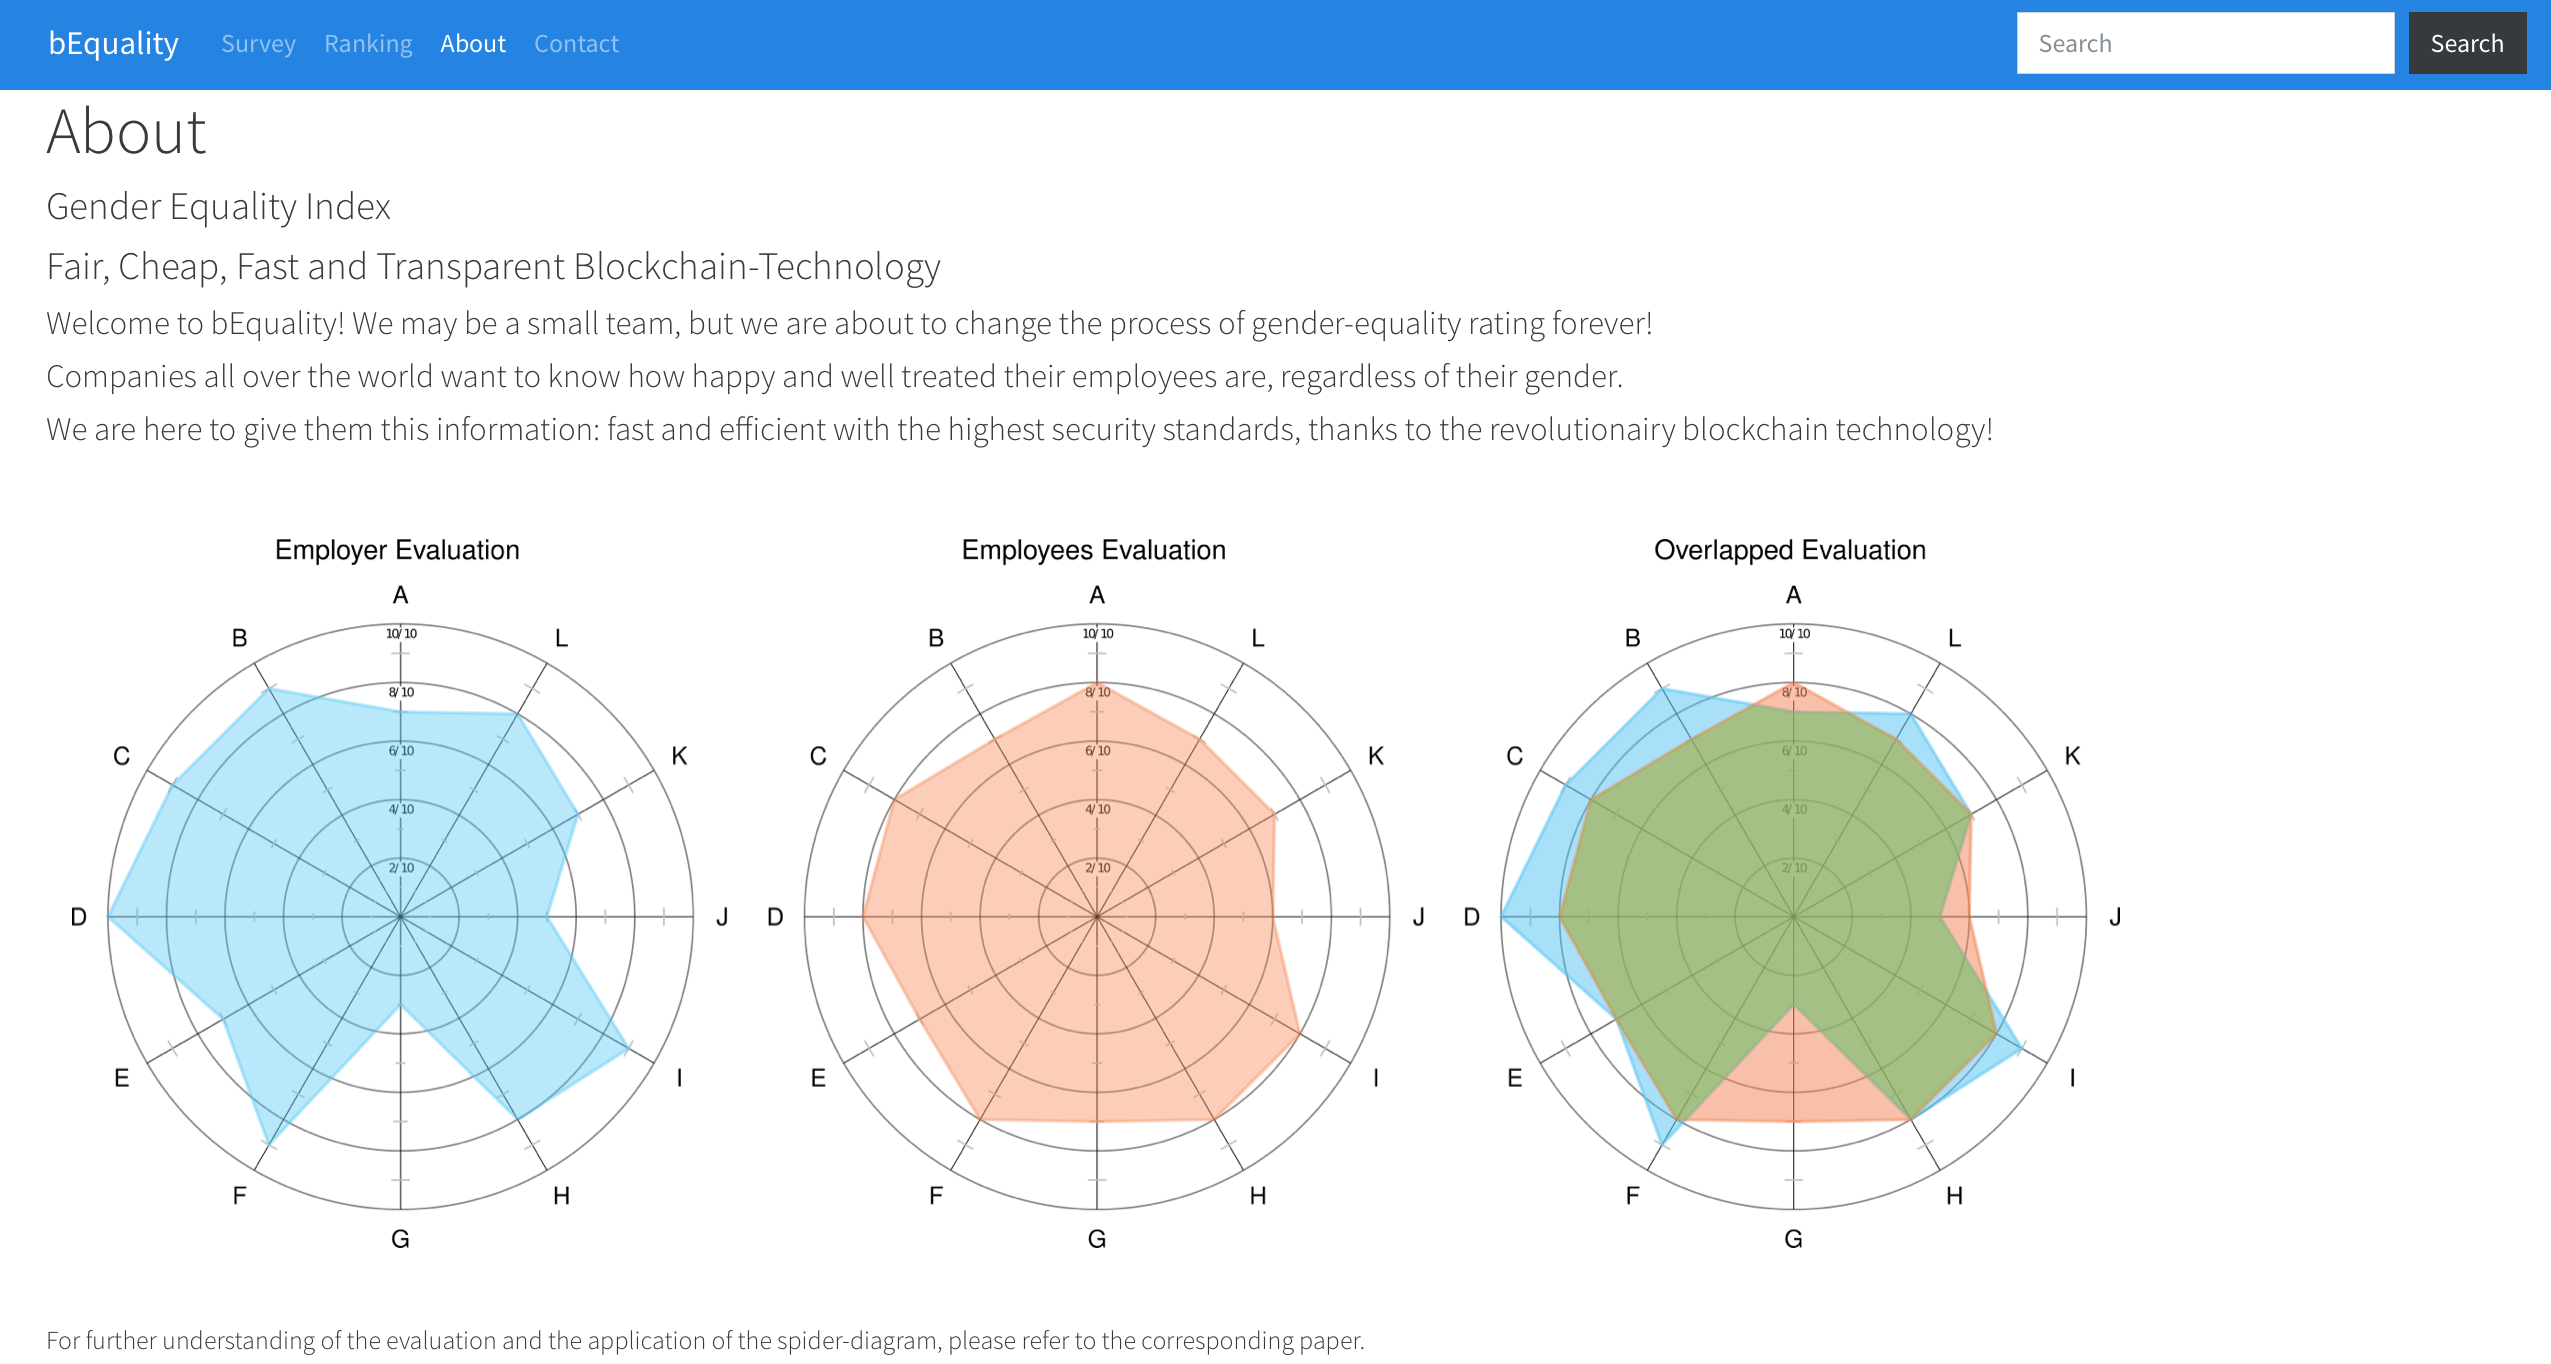
\includegraphics[width=0.7\textwidth]{Bilder/Website_3}
		\end{center}
		\begin{center}
			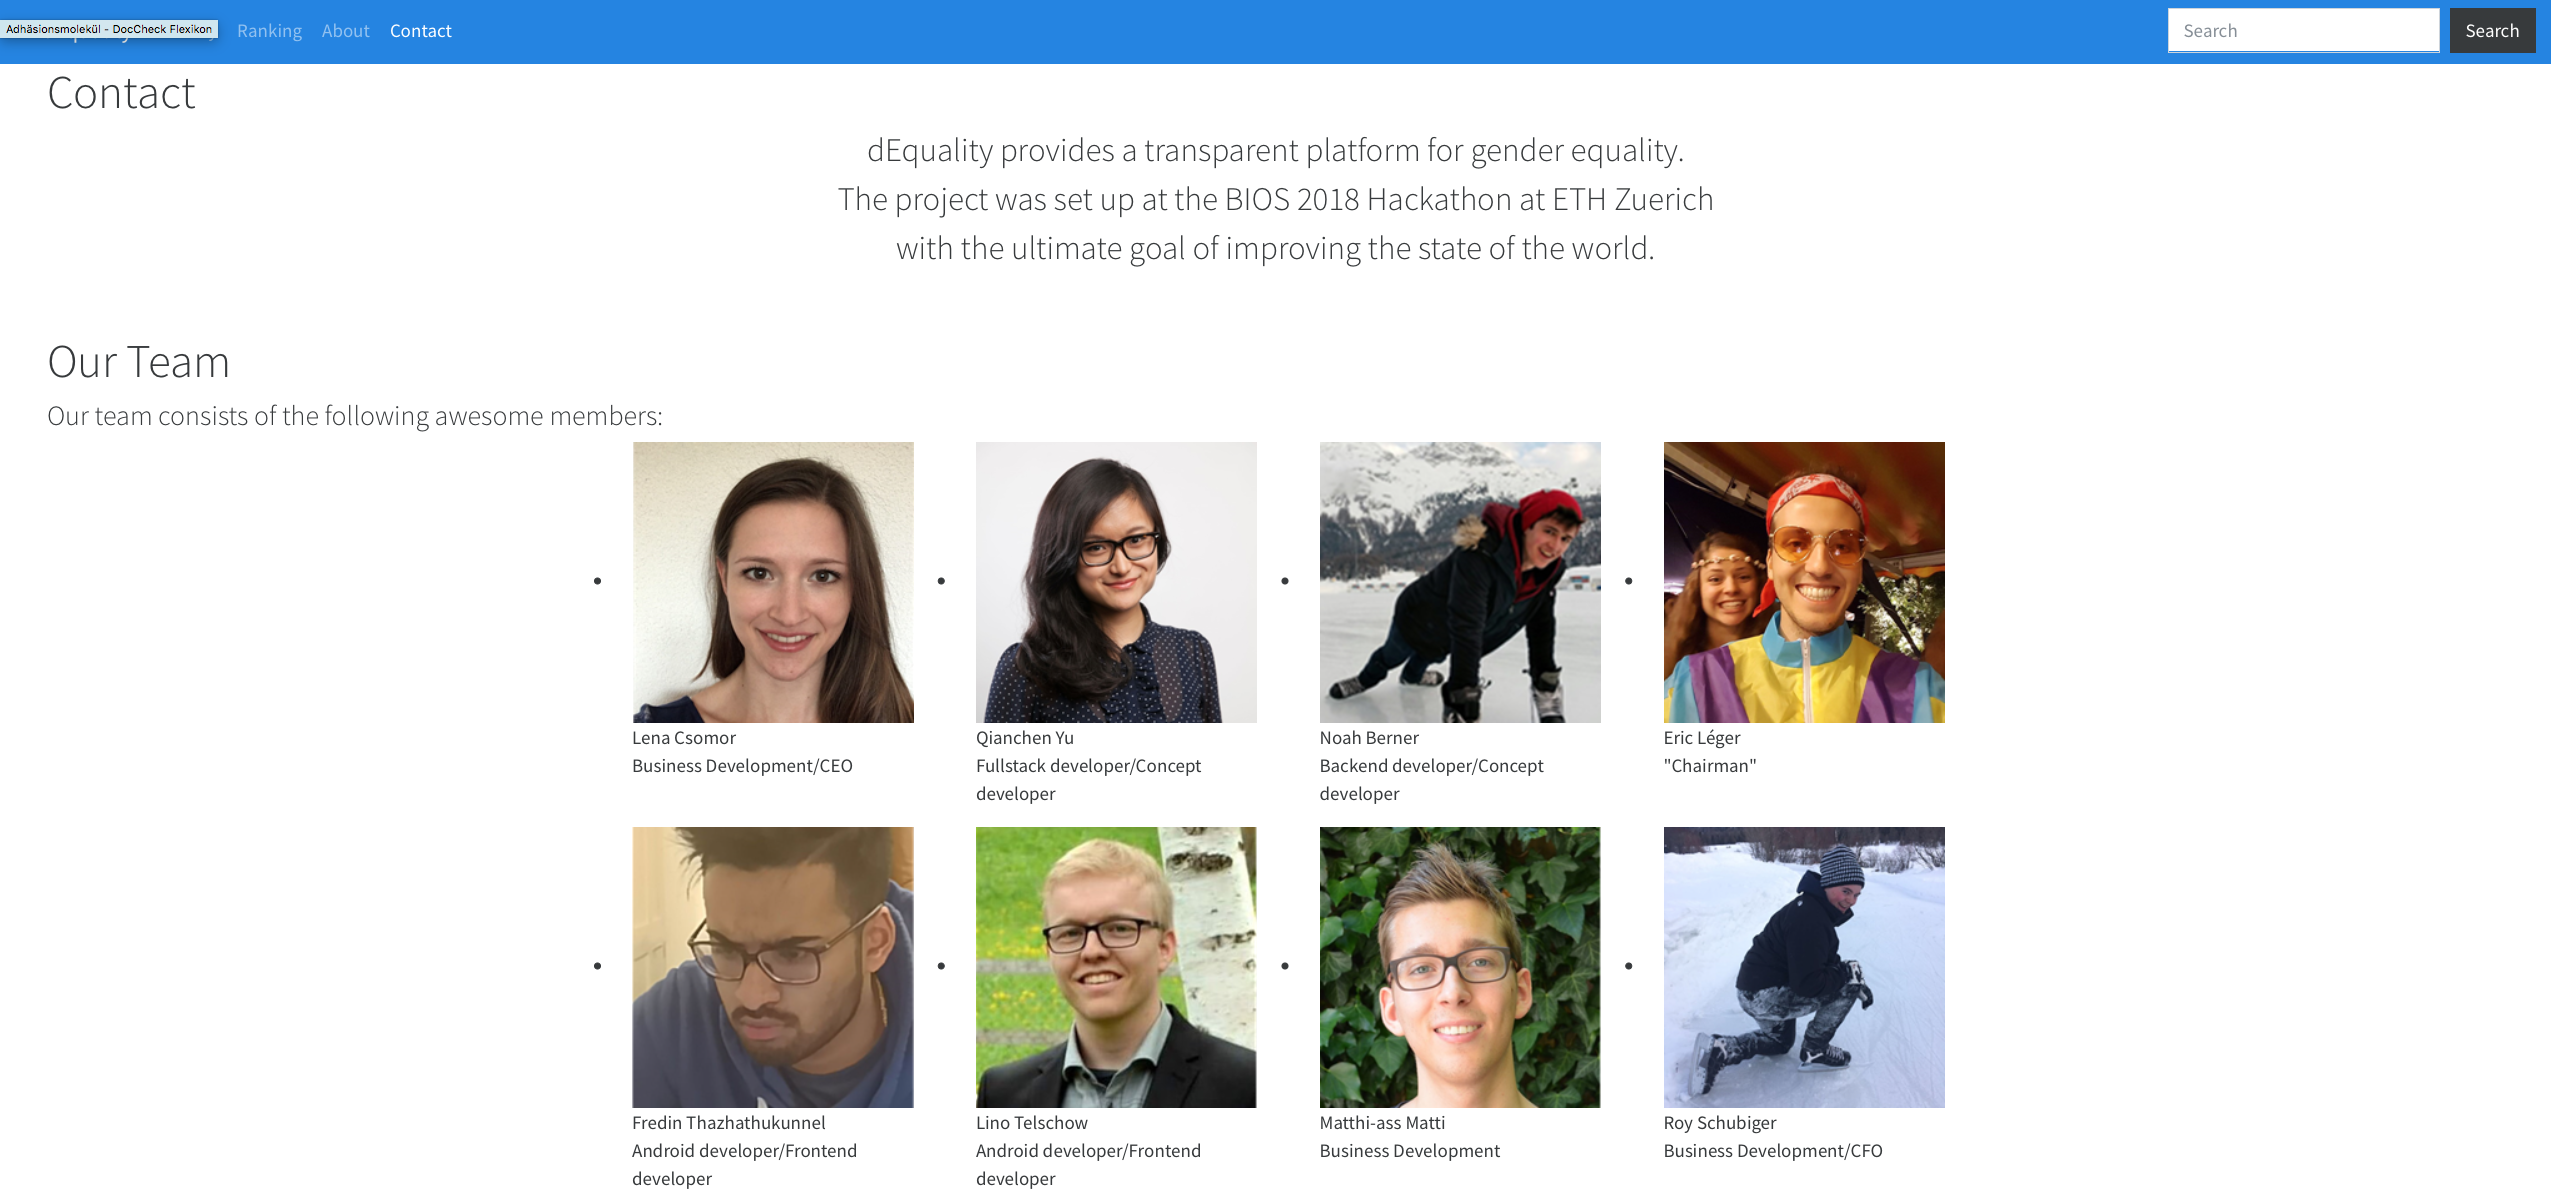
\includegraphics[width=0.7\textwidth]{Bilder/Website_4}
		\end{center}
	
	\subsection{E-Voting protocol}
		Below is a schematic way of our E-Voting protocol.
		\begin{figure}[H]
			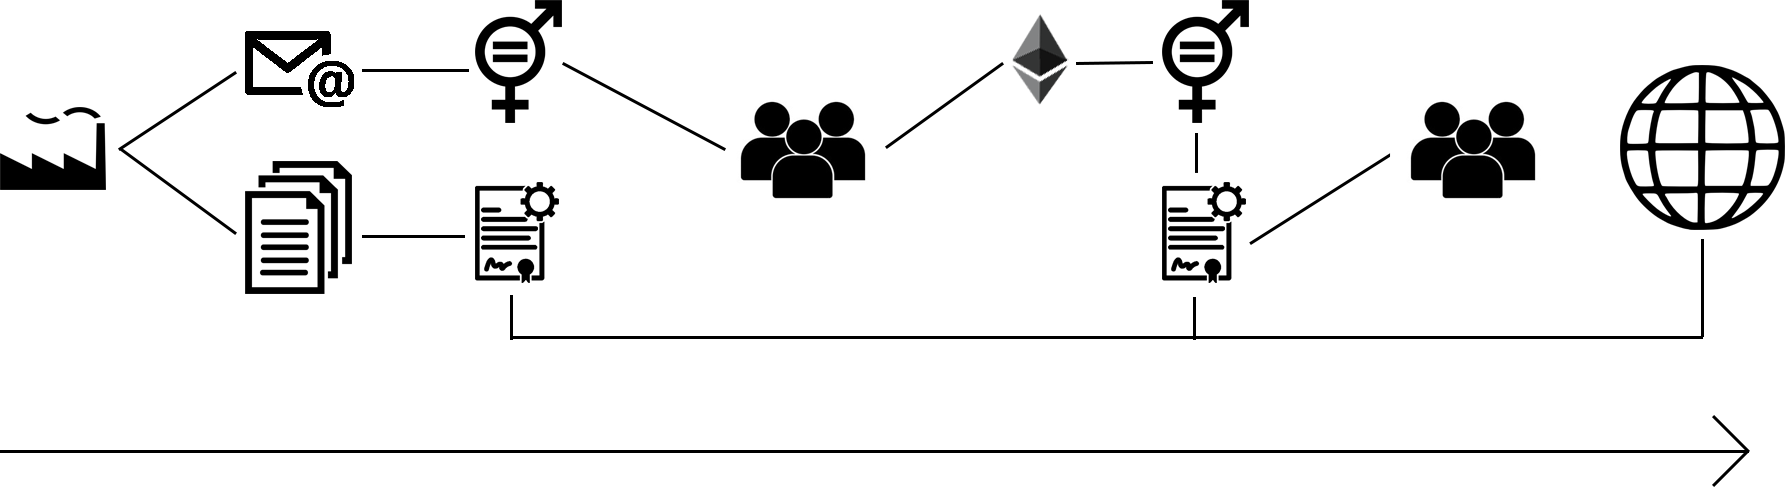
\includegraphics[width=0.9\textwidth]{Bilder/Survey_Protocol_preview_2}
			\caption{technical flow representation of the data capture and storage process}
			\label{technical_flow_representation}
		\end{figure}
	
	\subsection{\texttt{Survey.sol} Code}
		The SurveyFactory serves as a hub (deployed on the blockchain upon the launching of bEquality).\\
   		The company can create their own survey by providing a list of permitted user address.
   		\begin{lstlisting}
pragma solidity ^0.4.17;

contract SurveyFactory {

  //address owner;
  mapping(uint => address) public SurveyContracts;

  // function SurveyFactory(address adr) public {
  //    owner = adr;
  //}

  function createNewSurvey(uint companyID, address[] addressessOfEmployees, string _hashToaddressessOfEmployees) public returns(address newContract) {
    // require(msg.sender == owner);
    require(SurveyContracts[companyID] == 0x0);
    Survey c = new Survey(addressessOfEmployees, _hashToaddressessOfEmployees);
    SurveyContracts[companyID] = c;
    return c;
  }
  
  function getContractAddress(uint companyID) public constant returns (address) {
    return SurveyContracts[companyID];
  }
}
   		\end{lstlisting}
   		
   		The Survey contract is the child contract created by the SurveyFactory where only the permitted user can modify.
   		
   		\begin{lstlisting}
pragma solidity ^0.4.17;

contract Survey {
    mapping (address => string) public hashes;
    mapping (address => bool) public isAllowedToSumbitSurvey;
    string hashToaddressessOfEmployees;

    function Survey(address[] addressessOfEmployees, string _hashToaddressessOfEmployees) public {
        hashToaddressessOfEmployees = _hashToaddressessOfEmployees;
        for (uint256 index = 0; index < addressessOfEmployees.length; index++) {
            isAllowedToSumbitSurvey[addressessOfEmployees[index]] = true;
        }
    }

    function submitResults(string myHash) public {
        require(bytes(hashes[msg.sender]).length == 0);
        require(isAllowedToSumbitSurvey[msg.sender]);
        hashes[msg.sender] = myHash;
    }
}
		\end{lstlisting}

\clearpage

\end{document}
